\documentclass[tikz,border=2pt]{standalone}
% Preámbulo común de los diagramas TikZ (misma paleta y letra que las notas)
\usepackage[T1]{fontenc}\usepackage[utf8]{inputenc}
\usepackage{libertinus}\usepackage{libertinust1math}
\usepackage[defaultsans,scale=0.92]{lato}
\usepackage{amsmath,amssymb,bm}
\usepackage{tikz}\usetikzlibrary{calc,positioning,arrows.meta,shapes.geometric,decorations.pathreplacing,decorations.pathmorphing,fit,backgrounds}
\definecolor{snlazul}{HTML}{1E5AA8}\definecolor{snlnoche}{HTML}{14213D}\definecolor{snlvioleta}{HTML}{6C4AB6}
\definecolor{snlcoral}{HTML}{D1495B}\definecolor{snlambar}{HTML}{E09F3E}\definecolor{snlverde}{HTML}{2A9D8F}
\definecolor{snlteal}{HTML}{0F7173}\definecolor{snlgris}{HTML}{5C677D}\definecolor{snlfondo}{HTML}{F4F6FA}
\tikzset{>={Stealth[length=2.2mm]},
  bloque/.style={draw=#1,fill=#1!8,thick,rounded corners=2pt,minimum height=11mm,minimum width=20mm,align=center,font=\small},
  bloque/.default=snlazul,
  suma/.style={draw=snlnoche,thick,circle,inner sep=0pt,minimum size=5mm},
  flecha/.style={->,thick,draw=snlnoche},
  etq/.style={font=\small,text=snlnoche},
  nota/.style={font=\footnotesize\sffamily,text=snlgris,align=center}}

\begin{document}
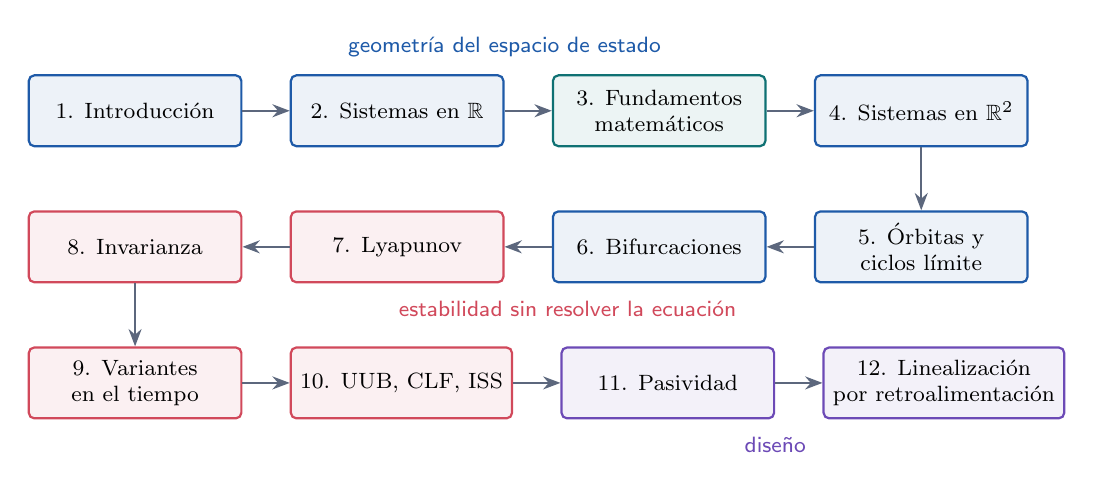
\begin{tikzpicture}[cap/.style={bloque=#1,minimum width=27mm,minimum height=9mm,font=\footnotesize},node distance=5mm and 6mm]
 % fila 1: geometría
 \node[cap=snlazul] (c1) {1. Introducción};
 \node[cap=snlazul,right=of c1] (c2) {2. Sistemas en $\mathbb{R}$};
 \node[cap=snlteal,right=of c2] (c3) {3. Fundamentos\\matemáticos};
 \node[cap=snlazul,right=of c3] (c4) {4. Sistemas en $\mathbb{R}^2$};
 % fila 2
 \node[cap=snlazul,below=8mm of c4] (c5) {5. Órbitas y\\ciclos límite};
 \node[cap=snlazul,left=of c5] (c6) {6. Bifurcaciones};
 \node[cap=snlcoral,left=of c6] (c7) {7. Lyapunov};
 \node[cap=snlcoral,left=of c7] (c8) {8. Invarianza};
 % fila 3: estabilidad avanzada y diseño
 \node[cap=snlcoral,below=8mm of c8] (c9) {9. Variantes\\en el tiempo};
 \node[cap=snlcoral,right=of c9] (c10) {10. UUB, CLF, ISS};
 \node[cap=snlvioleta,right=of c10] (c11) {11. Pasividad};
 \node[cap=snlvioleta,right=of c11] (c12) {12. Linealización\\por retroalimentación};
 \foreach \a/\b in {c1/c2,c2/c3,c3/c4,c4/c5,c5/c6,c6/c7,c7/c8,c8/c9,c9/c10,c10/c11,c11/c12}
   \draw[flecha,draw=snlgris] (\a) -- (\b);
 \node[nota,above=1mm of c2.north east,anchor=south] {\textcolor{snlazul}{geometría del espacio de estado}};
 \node[nota,below=1mm of c7.south east,anchor=north,xshift=8mm] {\textcolor{snlcoral}{estabilidad sin resolver la ecuación}};
 \node[nota,below=1mm of c11.south east,anchor=north] {\textcolor{snlvioleta}{diseño}};
\end{tikzpicture}
\end{document}
